\begin{figure}[H]
	\centering
	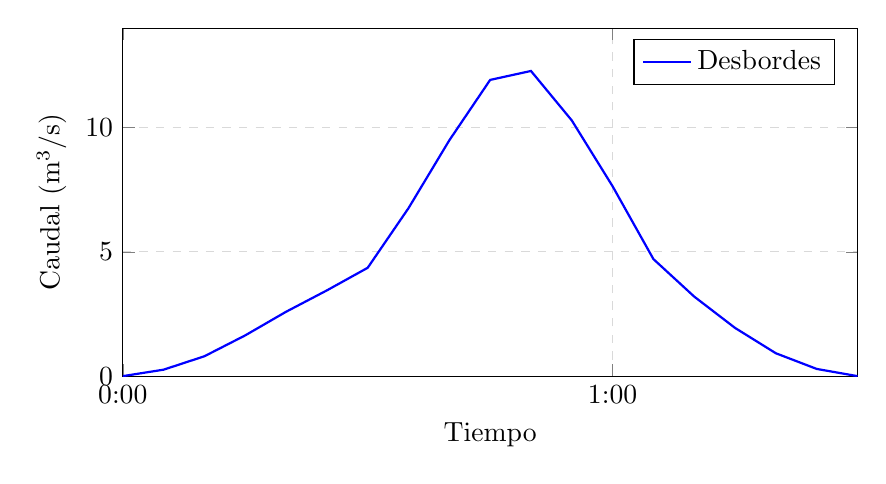
\begin{tikzpicture}
		\begin{axis}[
			width=0.9\textwidth,
			height=6cm,
			xlabel={Tiempo},
			ylabel={Caudal (m$^3$/s)},
			xmin=0,
			xmax=90,
			ymin=0,
			ymax=14,
			grid=major,
			grid style={dashed, gray!30},
			legend pos=north east,
			xtick={0, 60},
			xticklabels={0:00, 1:00},
			]
		% Desbordes
		\addplot [
		blue,
		thick,
		solid,
		] coordinates {
				(0, 0.00) (5, 0.26) (10, 0.80) (15, 1.64) (20, 2.59)
				(25, 3.45) (30, 4.36) (35, 6.76) (40, 9.49) (45, 11.92)
				(50, 12.28) (55, 10.29) (60, 7.64) (65, 4.71) (70, 3.20)
				(75, 1.94) (80, 0.92) (85, 0.29) (90, 0.00)
		};
		\addlegendentry{Desbordes}

		\end{axis}
	\end{tikzpicture}
	\caption{Hidrograma - Desbordes + BLOCKS $T_r$=25 años ($Q_p$=12.278 m$^3$/s)}
	\label{fig:hydro_desbordes_blocks_Tr25}
\end{figure}
